El microcontrolador PIC18F4550 posee un m\'etodo de grabaci\'on en
circuito\footnote{V\'ease -
\url{http://ww1.microchip.com/downloads/en/DeviceDoc/30277d.pdf}} (In-Circuit
Serial Programming). Esta prestaci\'on es implementada, no solo para dar
dinamismo al desarrollo, sino tambi\'en para permitir futuras actualizaciones
de firmware en las placas de producci\'on. Como se ve en la figura
\ref{fig:icsp}, la implementaci\'on de esta funcionalidad es bastante
sencilla.\\

\begin{figure}[htp]
\centering
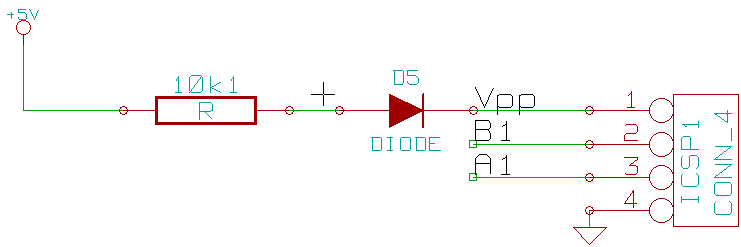
\includegraphics[width=7cm]{./img/icsp.png}
\caption{Conexi\'on ICSP (In-circuit Serial Programming)}
\label{fig:icsp}
\end{figure}

En cuanto a la velocidad de procesamiento, si bien el microcontrolador soporta
cristales externos de hasta 20 MHz, se usa uno de 4 MHz, ya que son los m\'as
com\'unmente usados y en algunos casos m\'as baratos.\\

%%%%%%%%%%%%%%%%%%%%%%%%%%%%%%%%%%%%
El microcontrolador posee varios registros de configuraci\'on que deben ser
escritos para habilitar ciertas funcionalidades.\
La configuraci\'on usada se aprecia en el siguiente pedazo de c\'odigo.

\begin{lstlisting}
code char at 0x300000 CONFIG1L = 0x20; /* USB clk 96MHz PLL/2, PLL 4MHz */
code char at 0x300001 CONFIG1H = 0x0e; /* HSPLL                         */
code char at 0x300002 CONFIG2L = 0x20; /* USB regulator enable, PWRT On */
code char at 0x300003 CONFIG2H = 0x00; /* Watchdog OFF                  */
code char at 0x300004 CONFIG3L = 0xff; /*         ***UNUSED***          */
code char at 0x300005 CONFIG3H = 0x81; /* MCLR enabled, PORTB digital   */
code char at 0x300006 CONFIG4L = 0x80; /* all OFF except STVREN         */
code char at 0x300007 CONFIG4H = 0xff; /*         ***UNUSED***          */
code char at 0x300008 CONFIG5L = 0xff; /* No code read protection       */
code char at 0x300009 CONFIG5H = 0xff; /* No data/boot read protection  */
code char at 0x30000A CONFIG6L = 0xff; /* No code write protection      */
code char at 0x30000B CONFIG6H = 0xff; /* No data/boot/table protection */
code char at 0x30000C CONFIG7L = 0xff; /* No table read protection      */
code char at 0x30000D CONFIG7H = 0xff; /* No boot table protection      */
\end{lstlisting}


%%%%%%%%%%%%%%%%
%%%%%%%%%%%%%%
%%%%%%%%%%%%
%%%%%%%%%%
%%%%%%%%
%%%%%%
%%%%%
%%%
Si bien no se encuentra dentro del alcance de este trabajo proveer una
soluci\'on para la parte mec\'anica de la impresora, es necesario determinar
con que debe interactuar la parte electr\'onica, esto es; cuales ser\'an las
entradas y cuales ser\'an las salidas.\\

Como se determin\'o anteriormente el mecanismo a usar ser\'a de un \'unico
punz\'on deslizante, esto implica que se debe generar movimiento horizontal
para el cabezal y movimiento vertical para el papel, es necesaria adem\'as una
se\~nal para manejar el punz\'on. Quedan entonces definidas las salidas.\
Por otra parte es necesario definir alg\'un tipo de se\~nal de entrada. Para
mantener un dise\~no simple solo se usar\'an entonces una se\~nal de presencia
de papel y un fin de carrera para el cabezal.\\

En la figura \ref{fig:pc_uc_motors} se ve el dise\~no general. \'Este posee la
particularidad de ser el usado por la mayor\'ia de las antiguas impresoras
matriz de punto, siendo entonces posible usar un mecanismo fabricado a medida,
o bien adaptar una impresora vieja.


\begin{figure}[htp]
\centering
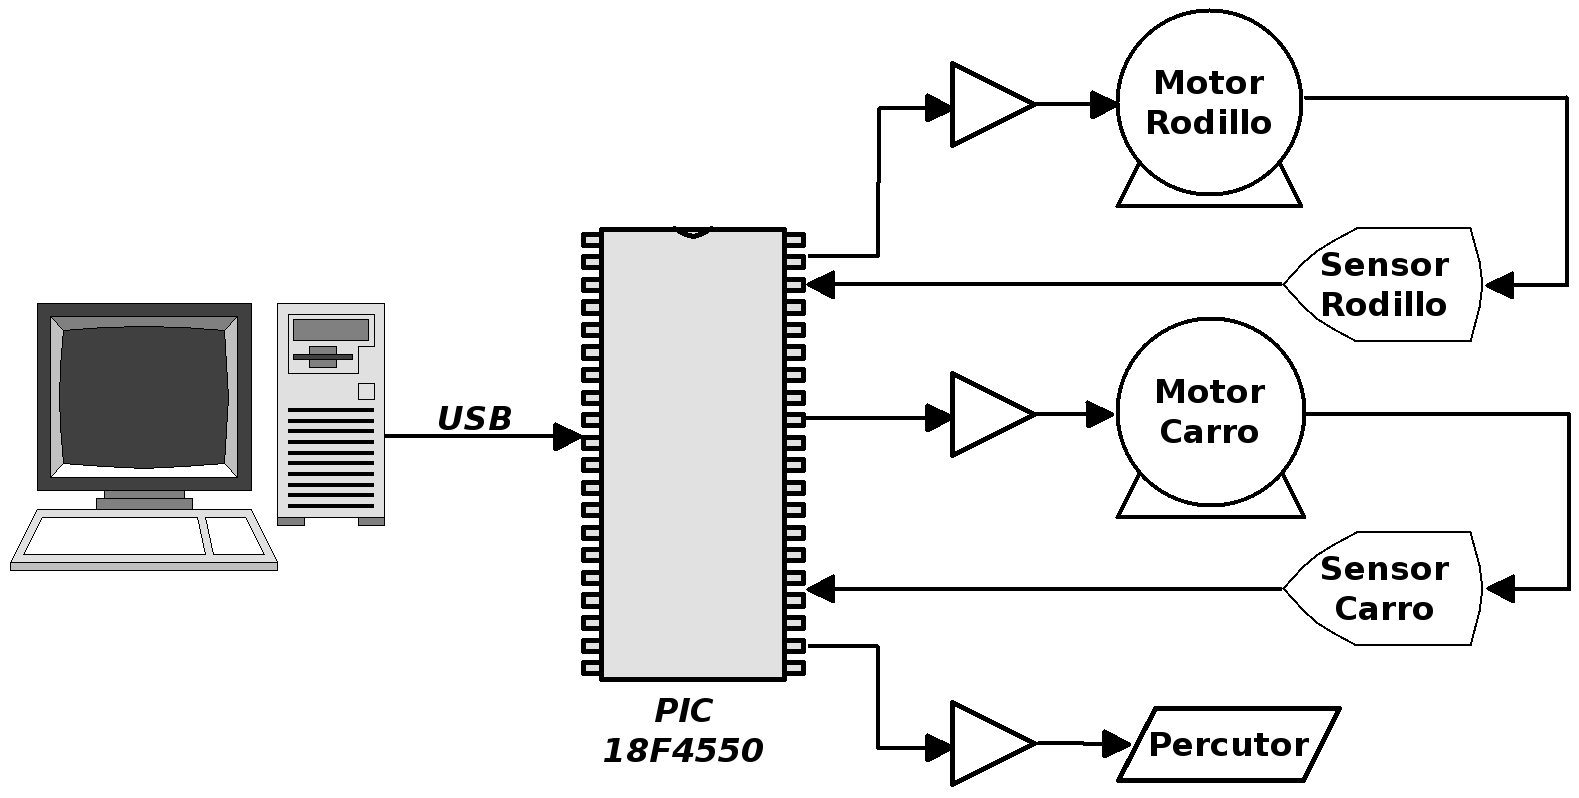
\includegraphics[width=13cm]{./img/pc_uc_motors.png}
\caption{Dise\~no de alto nivel.}
\label{fig:pc_uc_motors}
\end{figure}

Se implementan a modo de protecci\'on circuitos opto acoplados para la
entrada de los sensores y la salida del percutor. En la figura
\ref{fig:opto_percutor} se ve el circuito de la salida del percutor, y en la
figura \ref{fig:opto_sensor} el circuito de uno de los sensores. En ambos
casos se ha agregado un LED para ayuda visual.\\

\begin{figure}[htp]
\centering
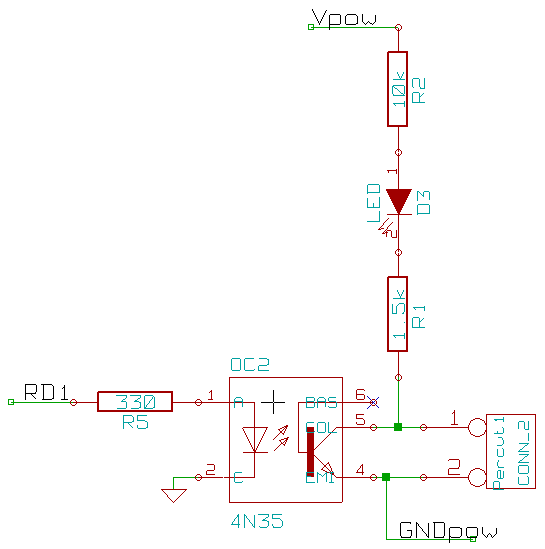
\includegraphics[width=7cm]{./img/opto_percutor.png}
\caption{Circuito opto acoplado para el percutor}
\label{fig:opto_percutor}
\end{figure}

\begin{figure}[htp]
\centering
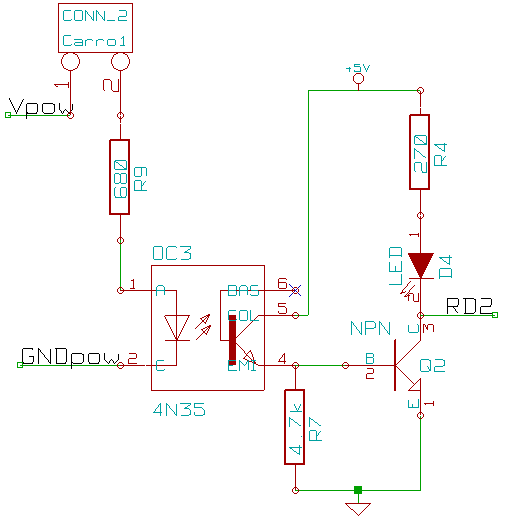
\includegraphics[width=7cm]{./img/opto_sensor.png}
\caption{Circuito opto acoplado para uno de los sensores}
\label{fig:opto_sensor}
\end{figure}



Para mantener los costos bajos, y teniendo en cuenta las limitaciones del
microcontrolador elegido, la mayor parte del procesamiento se lleva a cabo
en la computadora, logrando de esta manera economizar espacio en el firmware y
evitar la necesidad de hardware extra.\\

En su mayor\'ia, las impresoras braille comerciales posen integrado un sistema
sintetizador de voz, con mensajes pregrabados en varios idiomas que se
reproducen por cada acci\'on que la impresora ejecuta. Esto, claro est\'a,
implica la necesidad de grandes cantidades de memoria y quiz\'a un chip
dedicado. Para evitar usar chips sintetizadores de voz y memorias, y
teniendo en cuenta que la mayor\'ia de las computadoras actuales poseen
sistemas
de reproducci\'on de audio, \'este trabajo queda a cargo de \'estas.\
Al igual que el audio, existe gran cantidad de procesamiento a llevar a cabo
para la conversi\'on del texto a braille, y varias decisiones que usualmente
toman las impresoras. Todo esto se resuelve del lado de la computadora.\
Entonces es posible ahora, hablar de driver (que ser\'a el programa
ejecut\'andose en la computadora) y firmware (que ser\'a el programa
ejecut\'andose
en el microcontrolador) al referirnos a la computadora y a el dispositivo
respectivamente.\
Para lograr esto, el firmware solo es capaz de realizar tareas b\'asicas y
sencillas, respondiendo a instrucciones que el driver env\'ia y reportando los
resultados obtenidos. La figura \ref{fig:driver_firmware} muestra una
representaci\'on de lo dicho anteriormente.\\

\begin{figure}[htp]
\centering
\begin{tikzpicture}[node distance = 10cm, auto]
  \node [block] (driver) {Driver};
  \node [block, right of=driver] (firmware) {Firmware};
  \draw [line] (driver) to [bend right] node [midway] {Datos} (firmware);
  \draw [line] (driver) to [bend left] (firmware) node [midway]
{Instrucciones};
  \draw [line] (firmware) -- node [midway] {Resultados} (driver);
\end{tikzpicture}
\caption{Canales de comunicaci\'on entre el driver y el firmware.}
\label{fig:driver_firmware}
\end{figure}


Para instanciar el modelo anterior haciendo uso del m\'etodo de comunicaci\'on
elegido\footnote{Esto es el est\'andar USB}, se definen dos
endpoints\footnote{V\'ease \fullref{cap:usb_endpoints}} bidireccionales, uno
dedicado exclusivamente al env\'io de datos (endpoint 1 o EP1) y otro para
enviar
instrucciones y recibir resultados (endpoint 2 o EP2). La figura
\ref{fig:driver_eps_firmware} muestra la comunicaci\'on mediante endpoints.


\begin{figure}[htp]
\centering
\begin{tikzpicture}[node distance = 10cm, auto]
  \node [block] (driver) {Driver};
  \node [block, right of=driver] (firmware) {Firmware};
  \draw [line] (driver) (1.2,0.6) -- (8.8,0.6) node [midway] {Datos - EP1}
(firmware);
  \draw [line] (driver) (1.2,0) -- (8.8,0) node [midway] {Instrucciones - EP2
Out} (firmware);
  \draw [latex-] (firmware) (1.2,-0.6) -- (8.8,-0.6) node [midway]
{Resultados - EP2 In} (driver);
\end{tikzpicture}
\caption{Canales de comunicaci\'on entre el driver y el firmware mediante
endpoints.}
\label{fig:driver_eps_firmware}
\end{figure}

Habiendo definido los canales de comunicaci\'on y sus respectiva funciones, es
necesario determina el tipo y forma de los datos y las instrucciones a manejar.

\subsubsection{Datos}
%%%%%%%%%%%%%%%%%%
%
La cantidad de caracteres braille que entran en el ancho de una hoja A4, ronda
los 30 dependiendo del tama\~no de las sangr\'ias. Para dejar un margen se
eligen
28 caracteres. Teniendo en cuenta que los caracteres braille poseen dos
columnas de puntos\footnote{V\'ease \fullref{cap:braille_cell}} y que el
dato m\'inimo que se puede enviar por USB es de un byte\footnote{V\'ease
\fullref{cap:usb_byte}}, para completar una linea a lo ancho de una p\'agina de
una fila de puntos se necesitan:

\begin{center}
$28 caracteres * 2 puntos = 56 bits$\\
$56 bits / 8  = 7 bytes$
\end{center}

\begin{table}[ht]
\centering
\begin{tabular}{|c|c|c|} \hline
\braille{c} \braille{c} \braille{c} \braille{c} &
\braille{c} \braille{c} \braille{c} \braille{c} &
... 												 \\ \hline
byte 1 & byte 2 & ...\\ \hline
\end{tabular}
\caption{Bytes por puntos braille} 
\label{tab:bytes_braille}
\end{table}

Entonces el m\'aximo numero de bytes a enviar por linea es de 7 bytes.\

Para formar una fila completa de caracteres, es necesario realizar tres
env\'ios, ya que los caracteres braille poseen tres filas de
puntos\footnote{V\'ease \fullref{cap:braille_cell}}, lo cual genera 21 bytes
($7bytes*3$) por fila, y un total de 588 ($21bytes * 28filas$) bytes por
p\'agina ya que en una hoja A4 se suelen imprimir 28 filas de caracteres. 

\subsubsection{Instrucciones}
%%%%%%%%%%%%%%%%%%%%%%%%%%
%
Para limitar la capacidad de funcionalidades del dispositivo solo se
definen ocho instrucciones b\'asicas descriptas en la tabla
\ref{tab:instructions_set}.

\begin{table}[ht]
\centering
\begin{tabular}{|l|c|l|} 												\hline
\rowcolor[gray]{.9}
Instrucci\'on & Byte & Descripci\'on 								\\ 	\hline
RESET 		&	0x01	&	Resetea el cabezal	al punto de origen	\\	\hline
PRINT 		&	0x02	&	Imprime los datos						\\	\hline
MOV\_SHORT 	&  	0x03	&	Desplaza el cabezal entre puntos		\\	\hline
MOV\_LONG  	&  	0x04	&	Desplaza el cabezal entre caracteres	\\	\hline
ROT\_SHORT 	&	0x05	&	Rota el rodillo entre lineas			\\	\hline
ROT\_LONG   &	0x06	&	Rota el rodillo entre caracteres		\\	\hline
PULL\_PAPER	&	0x07	&	Rota el rodillo hasta sacar el papel	\\	\hline
STATUS		&	0x08	&	Pide el estado de los sensores			\\	\hline
\end{tabular}
\caption{Instrucciones de impresi\'on} 
\label{tab:instructions_set}
\end{table}

Este set de instrucciones proporcionan todas las funcionalidades necesarias
para poder llevar a acabo un proceso de impresi\'on normal.

\subsubsection{Resultados}
%%%%%%%%%%%%%%%%%%%%%%%
%
Se definen dos tipos de resultados distintos, uno que es devuelto cuando se
env\'ia la instrucci\'on \emph{STATUS} y otro que se genera siempre luego de un
env\'io de datos que consta en el dato recreado por la impresora, esto es solo
a
modo de verificaci\'on tipo \emph{echo}.\\

Ante una instrucci\'on del tipo \emph{STATUS}, el dispositivo lee los estados
de los dos sensores y genera un byte de reporte descripto en la tabla
\ref{tab:report_byte}.


\begin{table}[ht]
\centering
\begin{tabular}{|c|c|c|c|c|c|c|c|}									\hline
\multicolumn{8}{|c|}{Byte}										\\	\hline
x & x & x & x & x & x & 1/0 & 1/0 								\\ 	\hline
- & - & - & - & - & - & Sensor de cabezal & Sensor de papel		\\	\hline
\end{tabular}
\caption{Byte de reporte} 
\label{tab:report_byte}
\end{table}

Entonces dependiendo del estado de los dos bits menos significativos del byte
de reporte, el driver puede saber en que estado se encuentra la impresora.\\

El segundo tipo de resultado definido es el \emph{echo}. Cuando el driver
env\'ia datos para imprimir, la impresora comienza el proceso de impresi\'on y
recrea los datos recibidos seg\'un lo que hace, luego este dato recreado
se env\'ia de vuelta al driver quien comprar ambos datos y verifica que sean
iguales, la figura \ref{fig:rec_dat} muestra un diagrama simplificado de este
proceso.

\begin{figure}[htp]
\centering
\begin{scriptsize}
\begin{tikzpicture}
  [auto,
   decision/.style={diamond, draw=blue, thick, fill=blue!20,
                    text width=9em, text badly centered,
                    inner sep=1pt},
   block/.style   ={rectangle, draw=blue, thick, fill=blue!20,
                    text width=10em, text centered, rounded corners,
                    minimum height=4em},
   line/.style    ={draw, thick, -latex' ,shorten >=2pt},
   cloud/.style   ={draw=red, thick, ellipse,fill=red!20,
                    minimum height=2em}]
  \matrix [column sep=10mm,row sep=7mm]
  {
    % row 1
      \node [cloud] (driver)   		{Driver}; & 
		&
      \node [cloud] (firmware) 		{Firmware}; \\
    % row 2
	  \node [block] (dat_send_d)	{Env\'io del dato a imprimir \(\$dat_d\)};
&
		&
      \node [block] (dat_resv_f)	{Recepci\'on del dato \(\$dat_d\)}; \\
    % row 3
     	& &
      \node [block] (print) 		{Proceso de impresi\'on y
reconstrucci\'on del dato \(\$dat_d -> \$dat_f\)};  \\
    % row 4
	\node	[block]	(dat_resv_d)	{Recepci\'on del dato reconstruido
	\(\$dat_f\)};
		& &
	  \node [block] (dat_send_f)	{Env\'io del dato reconstruido
\(\$dat_f\)};
\\
  };
  \begin{scope}[every path/.style={draw, -latex'}]
    \path	(dat_send_d) -- (dat_resv_f) node [midway] {EP1 Out};
    \path	(dat_resv_f) -- (print);
    \path   (print)      -- (dat_send_f);
    \path   (dat_send_f) -- (dat_resv_d) node [midway] {EP2 In};;
  \end{scope}
\end{tikzpicture}
\end{scriptsize}
\caption{Proceso de reconstrucci\'on de datos}
\label{fig:rec_dat}
\end{figure}

\subsection{Manejo de motores}
%%%%%%%%%%%%%%%%%%%%%%%%%%%%%%
Como se explica en \fullref{cap:motors_section}, se requieren dos motores, lo
cual implica tener a disposici\'on ocho se\~nales de control. Para ello se hace
uso del puerto B del microcontrolador, el cual posee la particularidad de estar
provisto de resistencias de \emph{pull-up} programables. De esta manera los
dos motores pueden controlarse mediante la escritura de un \'unico puerto.\
La figura \ref{fig:uc_portb_motors} muestra la conexi\'on del puerto B del
microcontrolador a la ficha de se\~nales de los motores.


\begin{figure}[htp]
\centering
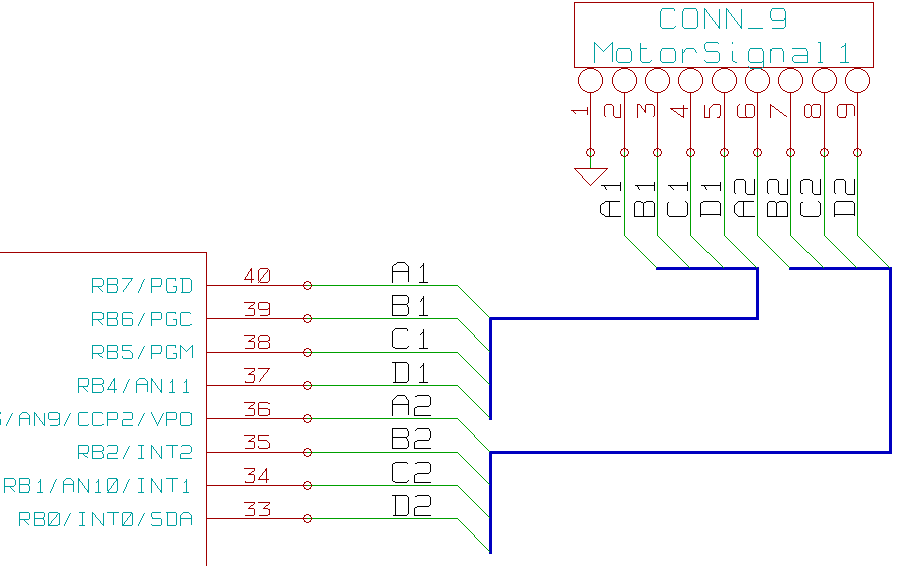
\includegraphics[width=7cm]{./img/uc_portb_motors.png}
\caption{Puerto B del uC conectado a las se\~nales de control de los motores
paso a paso.}
\label{fig:uc_portb_motors}
\end{figure}


Teniendo en cuenta la figura \ref{fig:stepper_motor_5_wire}, y tomando el
valor '1' como ``energizado'', las secuencias de la tabla
\ref{tab:seq_motors_1}, indistintamente, efect\'uan la rotaci\'on de el motor
en
un paso completo.

\begin{table}[htp]
\centering
\begin{tabular}{l c|c|c|c|c|}
Bobina A+ & & 1 & 0 & 0 & 0 \\	
Bobina B+ & & 0 & 0 & 1 & 0 \\
Bobina A- &	& 0 & 1 & 0 & 0 \\
Bobina B- &	& 0 & 0 & 0 & 1 \\
							\\
Bobina A+ & & 1 & 1 & 0 & 0 \\
Bobina B+ &	& 0 & 0 & 1 & 1 \\
Bobina A- &	& 0 & 1 & 1 & 0 \\ 
Bobina B- &	& 1 & 0 & 0 & 1 \\
							\\
Tiempo	...					\\
\end{tabular}
\caption{Secuencias de un paso para motores paso a paso unipolares de cuatro
fases.}
\label{tab:seq_motors_1}
\end{table}

Es posible combinar ambas secuencias para obtener incrementos de medio paso
como se ve en la tabla \ref{tab:seq_motors_2}, de esta manera se obtiene una
mejor precisi\'on en la rotaci\'on del motor.

\begin{table}[htp]
\centering
\begin{tabular}{l c|c|c|c|c|c|c|c|c|}
Bobina A+ & & 1 & 1 & 0 & 0 & 0 & 0 & 0 & 1\\	
Bobina B+ & & 0 & 0 & 0 & 1 & 1 & 1 & 0 & 0\\
Bobina A- &	& 0 & 1 & 1 & 1 & 0 & 0 & 0 & 0\\
Bobina B- &	& 0 & 0 & 0 & 0 & 0 & 1 & 1 & 1\\
							\\
Tiempo	...					\\
\end{tabular}
\caption{Secuencia de medio paso para motores paso a paso unipolares de cuatro
fases.}
\label{tab:seq_motors_2}
\end{table}



\clearpage
\begin{lstlisting}
/**
 * move() -     Function to move both motors
 * @loops:      Number of loops of a complete sequence
 * @direction:  Direction to move (RIGHT/LEFT, UP/DOWN)
 * @motor:      Which motor to move (CAR/ROLLER) 
 *
 * This function moves each motor in a defined direction and a specific
 * amount of turns depending on the parameters that are passed to it.
 **/
void move(byte loops, byte direction, byte motor) 
{
        byte stepsI[8] = {0x77, 0x33, 0xbb, 0x99, 0xdd, 0xcc, 0xee, 0x66};
        byte stepsD[8] = {0x66, 0xee, 0xcc, 0xdd, 0x99, 0xbb, 0x33, 0x77}; 
        byte val, i, loops_aux;

        if (direction)
                for (loops_aux = 0; loops_aux < loops; loops_aux++) {
                        for (i = 0; i < 8; i++) {		
                                val = stepsI[i];
                                if (motor) {
                                        PORTB = (PORTB & 0xf0) | (val & 0x0f);
                                        delay(50);
                                } else {
                                        PORTB = (PORTB & 0x0f) | (val & 0xf0);
                                        delay(50);
                                }
                        }
                }
        else
                for (loops_aux = 0; loops_aux < loops; loops_aux++) {
                        for (i = 0; i < 8; i++) {		
                                val = stepsD[i];
                                if (motor) {
                                        PORTB = (PORTB & 0xf0) | (val & 0x0f);
                                        delay(50);
                                } else {
                                        PORTB = (PORTB & 0x0f) | (val & 0xf0);
                                        delay(50);
                                }
                        }
                }
}
\end{lstlisting}


